\documentclass[a4paper,12pt]{article}
\usepackage{graphicx}
\usepackage[spanish]{babel}
\usepackage{geometry}
\usepackage{listings}
\usepackage{xcolor} % colores en codigo
\usepackage{wrapfig}   % Para permitir que el texto envuelva la imagen
%\usepackage[center]{background}
\geometry{left=2.54cm, right=2.54cm, top=2.54cm, bottom=2.54cm}
\renewcommand{\lstlistingname}{Código}
\lstdefinelanguage{JavaScript}{
  keywords={break, case, catch, continue, debugger, default, delete, do, else, finally, for, function, if, in, instanceof, new, return, switch, this, throw, try, typeof, var, void, while, with, let, const},
  keywordstyle=\color{blue}\bfseries,
  ndkeywords={class, export, boolean, throw, implements, import, this},
  ndkeywordstyle=\color{magenta}\bfseries,
  identifierstyle=\color{black},
  sensitive=true,
  comment=[l]{//},
  morecomment=[s]{/*}{*/},
  commentstyle=\color{gray}\ttfamily,
  stringstyle=\color{green!50!black},
  morestring=[b]',
  morestring=[b]"
}

\lstset{
  language=JavaScript,
  backgroundcolor=\color{gray!10},
  basicstyle=\ttfamily\footnotesize,
  numbers=left,
  numberstyle=\tiny\color{gray},
  stepnumber=1,
  numbersep=5pt,
  showstringspaces=false,
  breaklines=true,
  frame=single,
  tabsize=2,
}
\usepackage{setspace}
\usepackage{caption}   % Para subtítulos
\usepackage{float}  % Agregar en el preámbulo
\usepackage[colorlinks=true,linkcolor=black,urlcolor=blue]{hyperref}  % Para habilitar enlaces
\begin{document}
\thispagestyle{empty}

% --- Espacio superior ---
\vspace*{-1cm}

% --- Encabezado institucional ---
\begin{center}
\renewcommand{\baselinestretch}{2}\selectfont
\textbf{\LARGE UNIVERSIDAD AUTÓNOMA METROPOLITANA}\\[0.7cm]
\renewcommand{\baselinestretch}{1}\selectfont

    \textbf{\LARGE Unidad Cuajimalpa}\\[0.3cm]
    \textbf{\Large División de Ciencias Naturales e Ingeniería}\\[0.3cm]
    \textbf{\Large Licenciatura en Ingeniería en Computación}\\[2cm]
\end{center}
 
% --- Título del proyecto ---
\begin{center}
    \renewcommand{\baselinestretch}{2}\selectfont
        \textbf{\huge Punto de Venta Vinculado con un Bot de Discord}\\[0.7cm]
        \renewcommand{\baselinestretch}{1}\selectfont
    \textbf{\Large Proyecto Terminal}\\[3cm]
\end{center}

% --- Autor ---
\begin{flushleft}
    \textbf{\Large Autor:}\\[0.3cm]
    \textbf{\Large Álvaro Arturo Ramírez Arriaga}\\[2cm]
\end{flushleft}

% --- Asesores ---
\begin{flushleft}
    \textbf{\Large Asesores:}\\[0.3cm]
    \textbf{\Large Dr. José Netz Romero Durán}\\[0.2cm]
    \textbf{\Large Mtra. Núñez Reyes Alba Rocío}\\[2cm]
\end{flushleft}

% --- Fecha ---
\vfill
\begin{center}
    \textbf{\Large Ciudad de México, Agosto 2025}
\end{center}

\newpage

\tableofcontents
\newpage
\renewcommand\thesection{\arabic{section}}%reconfiguracion a arabico de las secciones

\section{Introducción}
  
\newpage

\subsection{Planteamiento del Problema}

 En la actualidad se ha visto un crecimiento en la preferencia de las personas por las redes sociales y plataformas de mensajería instantánea como Discord, que combina comunidad, mensajería y redes sociales. Actualmente, muchas tiendas envían actualizaciones importantes únicamente por correo, lo que resulta en que los mensajes se ignoren o queden en carpetas de spam.\\

Recientemente, las redes sociales han empezado a emplear mensajes automatizados o bots para agilizar las interacciones con los usuarios, evitando así que estos esperen a que una persona responda. Estos bots son software diseñado para realizar tareas específicas de forma repetida a una mayor velocidad que un ser humano; esto permite agilizar muchas tareas simples como enviar informes y/o mensajes.\\

Este proyecto planteó integrar un bot de Discord con una tienda en línea para centralizar la comunicación entre cliente y vendedor en la red social mencionada. Y así, abordar dos problemas clave: la dispersión de la comunicación y la falta de visibilidad de la información de compra.\\
 
El bot que se planteó para este proyecto pretendía realizar notificaciones en tiempo real sobre pagos, actualizaciones de pedidos y recordatorios de suscripciones, facilitando la visibilidad de la compra. Discord se ha convertido en un canal cotidiano para todo tipo de usuarios; para muchos, incluso mejora la experiencia respecto al correo electrónico, ofreciendo notificaciones instantáneas, interacción directa y personalización.\\

\newpage

\section{Objetivos}
En este apartado se presentan los objetivos planteados para guiar el desarrollo del proyecto y proponer una solución tecnológica para la gestión de compras y suscripciones mediante un bot de Discord.
\subsection{Objetivo General}
 Desarrollar un sistema de base de datos que permita el almacenamiento y consulta de los datos de compra a través de un bot de Discord. \\

\subsection{Objetivos Específicos}
Para este proyecto se tienen los siguientes objetivos específicos. \\

1.-  Desarrollar una base de datos que almacene y gestione la información de compras y suscripciones.\\

2.- Integrar un bot de Discord que permita realizar consultas a la base de datos.\\

3.- Desarrollar un sistema de notificaciones automatizadas.\\

4.- Evaluar las funcionalidades del sistema.\\

\newpage

\section{Estado del Arte}
Analizaremos sitios que cuenten con características o funcionalidades similares a las que usaremos para el proyecto que se va a desarrollar: las herramientas a analizar serán PayPal (forma de pago), bot de Discord MEE6, proyecto Tienda Virtual, Uniformes Escolares y Facebook Market.\\

\subsection{PayPal}

El método de pago de PayPal se basa principalmente en una implementación a través de su API, más que en el diseño de una interfaz propia. Esta API requiere información como la solicitud de pago, el precio del producto y la cuenta de PayPal a la que se debe depositar el dinero una vez que se complete la transacción. Por lo tanto, la única tarea que debe implementar el programador es la integración de la API y el botón para invocar el proceso de pago de PayPal.\\

\begin{figure}[ht]  % Entorno figure para insertar la imagen
    \centering  % Centrar la imagen
    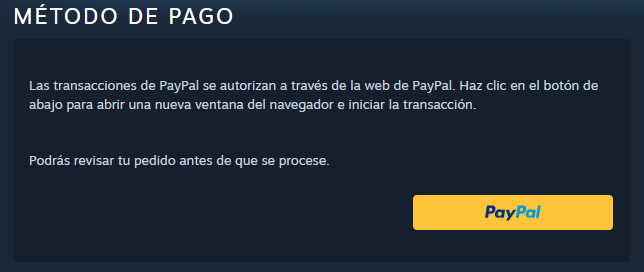
\includegraphics[width=0.7\textwidth]{./Imagenes/pago1.png} % Ajustar el tamaño de la imagen y la ruta de la imagen
    \captionsetup{justification=centering}
    \caption{Botón de método de pago PayPal.[1]}  % Pie de imagen o descripción
    \label{fig:pago1}  % Etiqueta para referenciar la imagen en el documento
\end{figure}

El botón de la figura 1 no es más que una conexión de la página web, la sección de pago con el verdadero gestor de la transacción, como es PayPal, mediante la API.

\newpage
Una vez llamada la API de PayPal, esta nos llevará a una ventana emergente (figura 2) donde se nos pedirá ingresar los datos de la cuenta de la plataforma PayPal para poder continuar con el cobro del servicio. Esta interfaz ya no es necesario crearla.\\

\begin{figure}[ht]  % Entorno figure para insertar la imagen
    \centering  % Centrar la imagen
    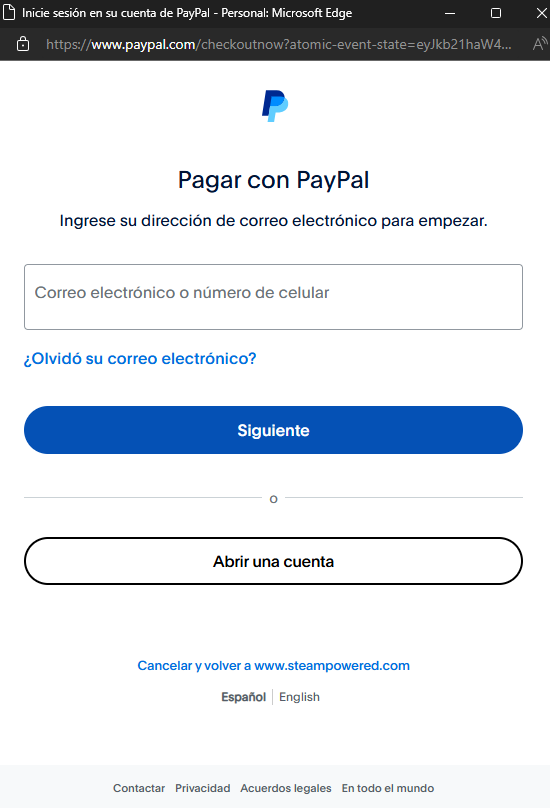
\includegraphics[width=0.5\textwidth]{./Imagenes/pago2.png} % Ajustar el tamaño de la imagen y la ruta de la imagen
    \captionsetup{justification=centering}
    \caption{Formulario dentro de PayPal para inicio de sesión.[1]}  % Pie de imagen o descripción
    \label{fig:pago2}  % Etiqueta para referenciar la imagen en el documento
\end{figure}

El pago entraría casi de inmediato, solo faltaría confirmar el pago para que se realice el cobro del servicio y finalizaría así el cobro por vía PayPal.

\newpage
\subsection{Meet 6 Bot Discord}

El bot que Meet 6 cuenta con muchas características interesantes para nosotros, pero en este proyecto nos centraremos en la posibilidad de enviar notificaciones de recordatorios por un canal en específico o por mensaje directo al usuario.

\begin{figure}[ht]  % Entorno figure para insertar la imagen
    \centering  % Centrar la imagen
    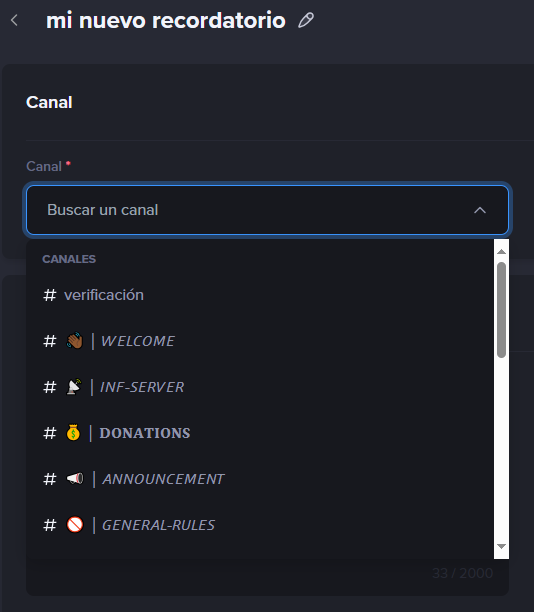
\includegraphics[width=0.6\textwidth]{./Imagenes/recordatorio1.png} % Ajustar el tamaño de la imagen y la ruta de la imagen
    \captionsetup{justification=centering}
    \caption{Ventana de selección de canal para generar el recordatorio.[2]}  % Pie de imagen o descripción
    \label{fig:recordatorio1}  % Etiqueta para referenciar la imagen en el documento
\end{figure}

En la ventana de la figura 3 podremos seleccionar en qué canal queremos que se genere el recordatorio que vamos a colocar. Esto es útil para aplicar recordatorios para un grupo de personas con roles en específico dentro del servidor de Discord. De esta forma. soloo llegarán los recordatorios a las personas que queremos quereciban estos mensajes. También podemos poner un auto rol para que ellos decidan si quieren recibir los recordatorios o no, algo similar a cuando te pregunta una empresa si quieres recibirr correos de promociones.

\begin{figure}[ht]  % Entorno figure para insertar la imagen
    \centering  % Centrar la imagen
    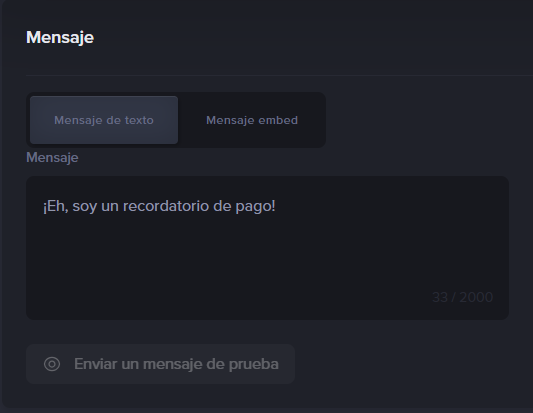
\includegraphics[width=0.6\textwidth]{./Imagenes/recordatorio3.png} % Ajustar el tamaño de la imagen y la ruta de la imagen
    \captionsetup{justification=centering}
    \caption{Ventana donde se ingresa el mensaje de recordatorio.[2]}  % Pie de imagen o descripción
    \label{fig:recordatorio2}  % Etiqueta para referenciar la imagen en el documento
\end{figure}
\newpage

En la ventana mostrada en la figura 4 se ingresará el mensaje que deseamos que los usuarios reciban como recordatorio. En este caso, el mensaje consistirá únicamente en texto, aunque también es posible agregar una imagen para que el bot la publique automáticamente junto con el texto. De esta forma, se puede generar una publicidad mucho más eficaz para los artículos y el público objetivo al que va dirigida.\\

Además, al tener la posibilidad de enviar mensajes directos a los usuarios, podremos notificarles sobre próximas fechas de pago para alguna suscripción activa, o incluso ofrecerles descuentos personalizados.

\newpage
\begin{figure}[ht]  % Entorno figure para insertar la imagen
    \centering  % Centrar la imagen
    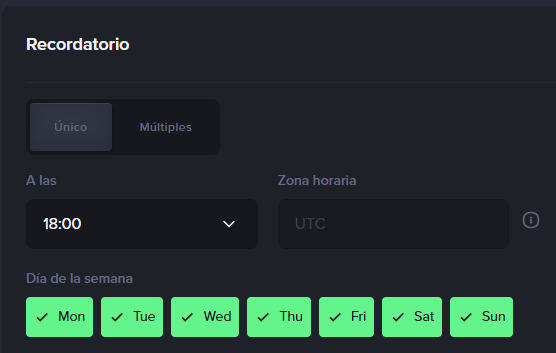
\includegraphics[width=0.7\textwidth]{./Imagenes/recordatorio2.png} % Ajustar el tamaño de la imagen y la ruta de la imagen
    \captionsetup{justification=centering}
    \caption{ventana de configuración de recordatorios automáticos.[2]}  % Pie de imagen o descripción
    \label{fig:recordatorio3}  % Etiqueta para referenciar la imagen en el documento
\end{figure}

La función de recordatorio se puede configurar de forma personalizada, como se muestra en la figura 5. Para que el recordatorio se genere automáticamente a intervalos de tiempo específicos, es necesario indicar el día y la hora. Esta funcionalidad es útil para evitar tener que crear el recordatorio de forma manual cada vez que se desee generar uno similar. En nuestro caso, tomará esta información de una base de datos, donde verificará si es necesario aplicar el recordatorio. En caso de tratarse de una mensualidad, recordará al usuario con 5 días de anticipación, revisando la fecha del siguiente cobro.
\newpage


\subsection{Tienda de Uniformes Escolares}

En este proyecto desarrollado en la universidad Oberta de Catalunya se realizó una tienda online de uniformes escolares, del cual tomaremos algunas utilidades de este proyecto como referencia.\\


\begin{figure}[ht]  % Entorno figure para insertar la imagen
    \centering  % Centrar la imagen
    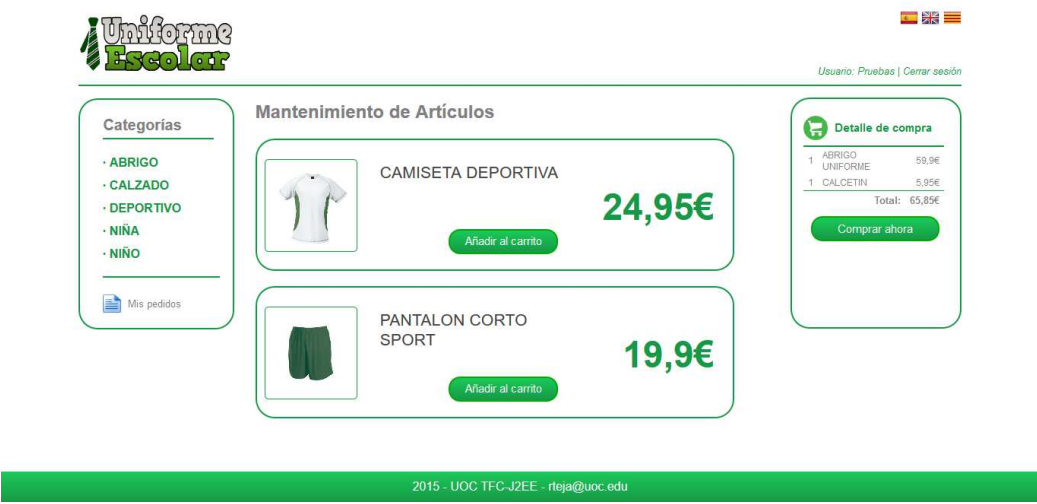
\includegraphics[width=0.8\textwidth]{./Imagenes/UE1.png} % Ajustar el tamaño de la imagen y la ruta de la imagen
    \captionsetup{justification=centering}  % Ajusta el caption para centrarlo
    \caption{Interfaz de artículos del proyecto tienda virtual de uniformes escolares.[3]\\} 
    \label{fig:ue1}  % Etiqueta para referenciar la imagen en el documento
\end{figure}

 Como podemos ver en la figura 6, en la interfaz de compra únicamente hace falta dar clic sobre ‘añadir al carrito’ para poder adquirirlo; también se ve el precio del producto y su nombre.\\

 Del lado izquierdo también se puede apreciar el filtro que se tiene para los productos, de esta forma se tiene una mejor organización sobre lo que está observando el usuario comprador en este momento. Al lado derecho se muestran los productos que han sido añadidos al carrito, así como el precio final de la compra.
 \newpage
 
  En la figura 7 podemos ver qué pasa al darle clic a comprar, ahora nos manda a la página de pago  donde saldrán los datos del comprador, en este caso se ve cómo el pago se carga automáticamente a la mensualidad del colegio, en nuestro caso habrá un método de pago para realizar el pago.\\
  
\begin{figure}[ht]  % Entorno figure para insertar la imagen
    \centering  % Centrar la imagen
    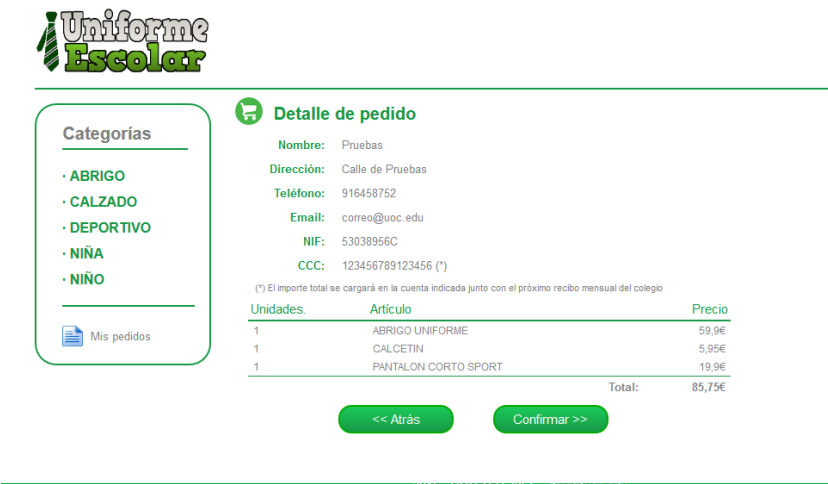
\includegraphics[width=0.8\textwidth]{./Imagenes/UE2.png} % Ajustar el tamaño de la imagen y la ruta de la imagen
    \captionsetup{justification=centering}
    \caption{ventana donde se muestra toda la información del comprador y la lista de lo que se está comprando.[3]}  % Etiqueta para referenciar la imagen en el documento
    \label{fig:ue2}  % Etiqueta para referenciar la imagen en el documento
\end{figure}

 Para nuestro proyecto será importante colocar una sección de productos para seleccionarlos y, después de seleccionarlos, colocar una descripción y más imágenes para que el comprador pueda ver y estar más seguro de que se está comprando, al igual que un desglose de su compra total.
\newpage
\clearpage
\subsection{Facebook Market}
Facebook Market también es otra de las plataformas más utilizadas para la compra y venta de productos, por esta razón es una buena referencia para el proyecto.\\

En la figura 8 podemos ver cómo se muestra la información del vendedor, detalles del producto y algunas especificaciones básicas; no es tan extensa la descripción como en Amazon. Sin embargo, nos da la posibilidad de enviarle un mensaje al comprador para poder preguntarle a él de una forma más directa y personalizada.\\

\begin{figure}[ht]
    \centering
    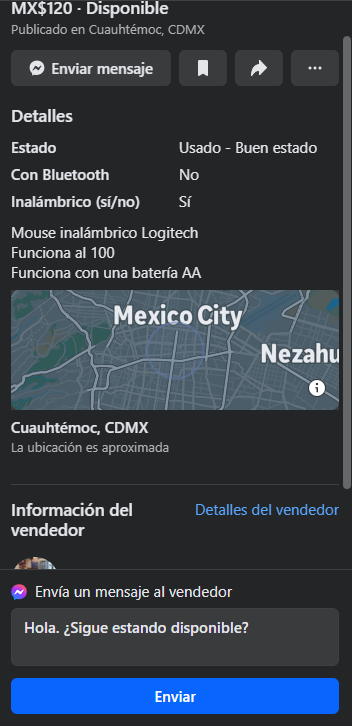
\includegraphics[width=0.35\textwidth]{./Imagenes/FBm3.png}
    \caption{Ventana de información del producto y del vendedor.[4]}
    \label{fig:fbm3}
\end{figure}

Si bien esta plataforma está orientada a que terceros vendan sus productos en su tienda, son buenas referencias para este proyecto, al poder tener un trato directo con el vendedor.\\

Este proyecto tomará la idea de poder mandarle mensajes directamente al vendedor, en este caso, el administrador de la tienda, para algunas compras que requieran de más pasos y no solo vender el producto.
\newpage
\subsection{AliExpress}
Algunas tiendas en línea ya utilizan actualmente notificaciones por medio de alguna red social; este es el caso de AliExpress, donde reenvían información básica de tu compra y links para visualizar la información completa de la compra en una página web. Si bien no es el ticket, sí facilita poder verlo sin necesidad de entrar al correo electrónico.\\

Este proyecto busca poder realizar notificaciones mediante una red social como es Discord para centralizar la forma de encontrar la información de compra y contactar con la tienda o persona encargada de esta de una forma mucho más fácil, utilizando únicamente Discord.
\begin{figure}[ht]
    \centering
    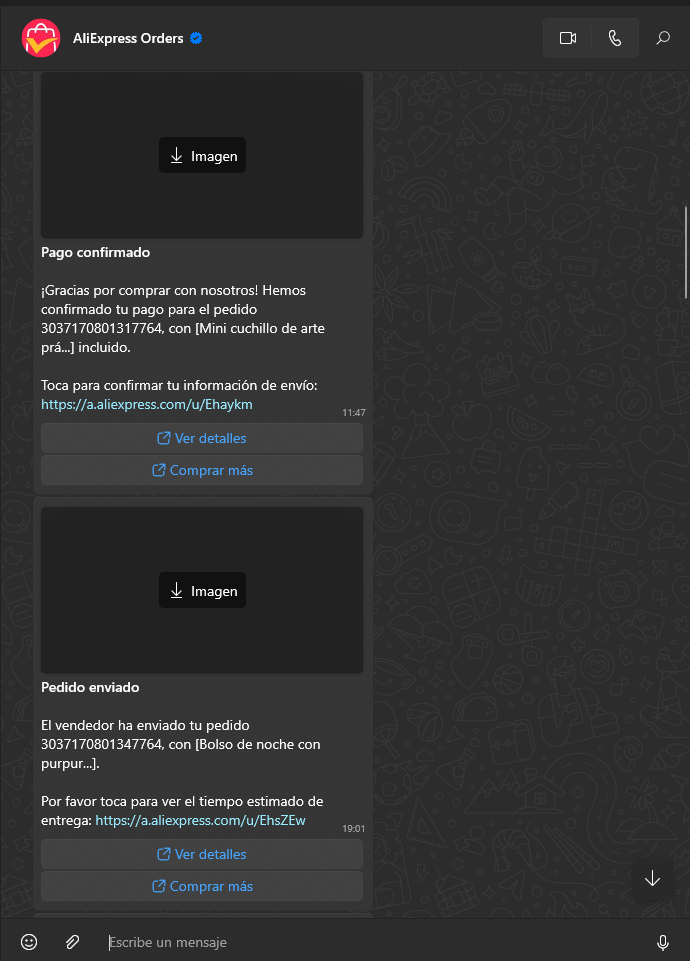
\includegraphics[width=0.5\textwidth]{./Imagenes/aliex.PNG}
    \caption{Información de compra recibida vía WhatsApp de AliExpress.[5]}
    \label{fig:aliex}
\end{figure}




\newpage


\section{Definición General del sistema}
\subsection{Propuesta}
Este proyecto propone el desarrollo de un sistema integrado con un bot de Discord para una tienda en línea, con el fin de centralizar la comunicación y optimizar la gestión de compras y suscripciones. A diferencia de otras soluciones existentes, la propuesta aprovecha la versatilidad y popularidad de Discord como plataforma para ofrecer notificaciones en tiempo real sobre pagos, actualizaciones de pedidos y recordatorios, mejorando la visibilidad y la interacción directa con los usuarios.\\

El sistema incluye el diseño y desarrollo de una base de datos robusta para almacenar y consultar información relevante, la integración del bot para realizar consultas y notificaciones automatizadas, y una interfaz administrativa que facilita la gestión de artículos, compras y suscripciones. Así, se busca proporcionar una solución tecnológica adaptada a las necesidades específicas de la tienda, que combine eficiencia, usabilidad y aprovechamiento de plataformas de comunicación actuales.
\newpage
\subsection{Tecnologías}

Las tecnologías para este proyecto serán API PayPal, API Discord, 
 MYSQL, PHP, Node.js, React. Se explicará cada una de las tecnologías para definir qué funcionalidad van a desempeñar en el proyecto propuesto.
\subsubsection{PayPal}

PayPal es una de las plataformas más populares para pagos en línea, conocida por su facilidad de uso, seguridad y aceptación internacional. Para este proyecto, se ha elegido PayPal debido a su amplia adopción por los usuarios y su capacidad para gestionar pagos transfronterizos de manera eficiente, ofreciendo una ventaja frente a competidores como Mercado Pago.\\

La integración de PayPal en una tienda en línea se realiza principalmente mediante su API. Esta API permite establecer la comunicación entre la tienda y los servidores de PayPal para gestionar las transacciones de manera segura. Los pasos básicos para utilizar PayPal como método de pago son:\\


\subsubsection{Discord}

Discord es una plataforma de comunicación ampliamente utilizada para la creación y gestión de comunidades temáticas. Originalmente orientada hacia los jugadores, Discord ha evolucionado para ser una herramienta versátil que permite administrar grandes grupos de usuarios gracias a su estructura basada en servidores. En estos servidores, se pueden asignar roles, gestionar permisos y utilizar bots para automatizar diversas tareas, convirtiéndola en una solución ideal para centralizar la interacción entre usuarios y servicios.\\

Discord será una herramienta central en este proyecto, gracias a su capacidad para gestionar usuarios y automatizar notificaciones. Se aprovecharán tanto su API como las características de inicio de sesión para integrar la tienda en línea con la plataforma.\\

Se utilizará la OAuth2 API de Discord para implementar un sistema de autenticación seguro y sencillo. Esto permitirá a los usuarios iniciar sesión en la tienda en línea con su cuenta de Discord, sin necesidad de crear un nuevo usuario.
\newpage

\subsubsection{Node.js}


Node.js es un entorno de ejecución que permite ejecutar JavaScript fuera del navegador. Basado en el motor V8 de Google Chrome, Node.js es extremadamente rápido y eficiente, especialmente para aplicaciones que requieren manejo en tiempo real.\\

Node.js es ideal para aplicaciones que necesitan manejar múltiples solicitudes simultáneamente, como un bot de Discord que responde a eventos en tiempo real. También tiene una muy buena estabilidad, por lo cual aunque haya muchas solicitudes simultáneas conserva un buen rendimiento.\\

Para este proyecto utilizaremos Node.js junto con una biblioteca llamada discord.js que simplifica la interacción con la API de Discord, la cual nos permitirá programar un bot que pueda enviar y recibir mensajes.\\ 

Esta api nos dará la posibilidad de asignar o modificar roles de usuarios automáticamente según ciertas condiciones. También nos dará la facilidad de que el bot pueda enviar mensajes directos, incrustaciones (embeds) con diseño visual atractivo, y notificaciones personalizadas.\\

Usando Discord.js, el bot enviará mensajes automáticos a los usuarios tras completar una compra, actualizando estados de pedidos o recordando renovaciones de suscripciones.
\subsubsection{React}

React es una biblioteca de JavaScript desarrollada por Facebook, diseñada para construir interfaces de usuario (UI) modernas, interactivas y dinámicas. Se enfoca principalmente en la creación de aplicaciones a través de componentes reutilizables, lo que permite dividir la interfaz en pequeñas piezas independientes y manejables. Esto mejora la organización y el mantenimiento del código; también facilita la reutilización de estos componentes en diferentes partes de la aplicación. En este proyecto, un componente podría encargarse de mostrar los productos de la tienda, otro del carrito de compras y otro de las notificaciones de compra, optimizando así el desarrollo.\\

Una de las características más destacadas de React es el uso del Virtual DOM. Este mecanismo crea una representación en memoria del DOM real, lo que permite que React identifique y actualice solo las partes necesarias de la interfaz en lugar de renderizarla por completo cada vez que hay un cambio. Esto mejora significativamente el rendimiento de la aplicación, especialmente en escenarios donde las actualizaciones en tiempo real son frecuentes, como al agregar productos al carrito o actualizar el estado de un pedido.\\

React fue elegido para este proyecto debido a su escalabilidad y facilidad de mantenimiento. React ofrece un equilibrio ideal entre flexibilidad y robustez, lo que lo convierte en una herramienta esencial para construir una tienda en línea moderna que integre funcionalidades avanzadas como notificaciones en tiempo real y bots automatizados.
\newpage
\subsubsection{MySQL}

MySQL es un sistema de gestión de bases de datos relacional, se utiliza para almacenar, organizar y administrar grandes volúmenes de información en aplicaciones de software. Este sistema utiliza el lenguaje SQL (Structured Query Language) para interactuar con los datos, permitiendo realizar operaciones como consultas, inserciones, actualizaciones y eliminaciones de manera eficiente y estructurada. \\

Una de las principales ventajas de MySQL es su capacidad para manejar grandes cantidades de datos de manera rápida y eficiente. Gracias a su diseño optimizado, MySQL permite realizar consultas complejas que filtran y procesan información específica en cuestión de milisegundos. Esto es crucial en aplicaciones como tiendas en línea, donde se manejan continuamente datos relacionados con usuarios, productos, pedidos y transacciones.\\

Otra característica importante de MySQL es su enfoque en la integridad de los datos y la seguridad. A través de herramientas como Prepared Statements (consultas preparadas), es posible proteger la base de datos contra ataques comunes como la inyección SQL, garantizando que las consultas se ejecuten de forma segura y controlada. Esta funcionalidad es esencial en proyectos que manejan información confidencial, como detalles de usuarios y transacciones económicas.\\

En este proyecto, MySQL se utilizará para gestionar tablas que almacenen información esencial como detalles de los usuarios, productos, pedidos y estados de pago. Además, permitirá realizar operaciones frecuentes, como buscar productos según filtros personalizados, actualizar el estado de un pedido en tiempo real o registrar nuevas transacciones.\\
\newpage
\subsection{Requerimientos Funcionales}
A continuación, se presentan los requerimientos funcionales del proyecto, los cuales describen las acciones y comportamientos que el sistema deberá cumplir para satisfacer las necesidades del usuario y alcanzar los objetivos planteados. Estos requerimientos definen qué funciones específicas realizará el sistema, incluyendo la interacción con el bot de Discord, la gestión de pedidos y la comunicación con los clientes.\\

\subsubsection{Página Web}

- Permitir a los usuarios navegar por los productos disponibles en la tienda virtual.\\

- Permitir a los usuarios autenticarse mediante Discord (OAuth2).\\

- Permitir a los usuarios agregar productos al carrito de compras.\\

- Permitir a los usuarios modificar la cantidad de productos en el carrito y eliminar productos del mismo.\\

- Permitir a los usuarios realizar compras y generar tickets de compra usando PayPal.\\

- Mostrar notificaciones de éxito o error en las operaciones principales (login, agregar al carrito, compra).\\

- Permitir a los usuarios ver su perfil y cerrar sesión.\\

- Mostrar información relevante de los productos (nombre, imagen, precio, categoría).\\

- Permitir la navegación entre diferentes páginas (productos, carrito, perfil).\\

- Integración con un servidor de Discord (botón de invitación y QR).\\

\subsubsection{Bot Discord}
- Permitir la integración con el servidor de Discord de la tienda virtual.\\

- Responder a comandos básicos de los usuarios /productos .\\

- Notificar en canales específicos cuando se realiza una compra o se genera un ticket en la tienda.\\

- Permitir la gestión de roles o permisos para usuarios que compran productos.\\

- Permitir la consulta de información de productos o tickets desde Discord (si aplica).\\
\newpage
\subsection{Requerimientos no Funcionales}
En esta sección se detallan los requerimientos no funcionales del proyecto, los cuales establecen los criterios de calidad que el sistema debe cumplir.
\subsubsection{Página Web}

- La aplicación debe ser responsiva y funcionar correctamente en dispositivos móviles y de escritorio.\\

- El sistema debe mantener la sesión del usuario mediante cookies seguras.\\

- El backend debe manejar la autenticación de manera segura.\\

- El sistema debe manejar errores y mostrar mensajes claros al usuario.\\

- El sistema debe ser escalable para permitir la integración de nuevas funcionalidades (por ejemplo, más métodos de pago, más categorías).\\

- El sistema debe proteger los datos sensibles y cumplir con buenas prácticas de seguridad.\\

- El backend debe soportar concurrencia y múltiples usuarios simultáneos.\\

- El sistema debe permitir la integración con servicios externos como Discord y PayPal.\\

\subsubsection{Bot Discord}\
- El bot debe estar disponible 24/7 y manejar desconexiones de manera automática.\\

- El código debe estar organizado y documentado para facilitar el mantenimiento.\\

- El bot debe manejar errores y excepciones sin interrumpir su funcionamiento.\\

- El bot debe proteger los tokens y credenciales de acceso.\\

- El bot debe ser escalable para permitir la adición de nuevos comandos o integraciones.\\
\newpage

\section{Diseño del Sistema}
\subsection{Diagrama General}

\begin{figure}[ht]  % Entorno figure para insertar la imagen
    \centering  % Centrar la imagen
    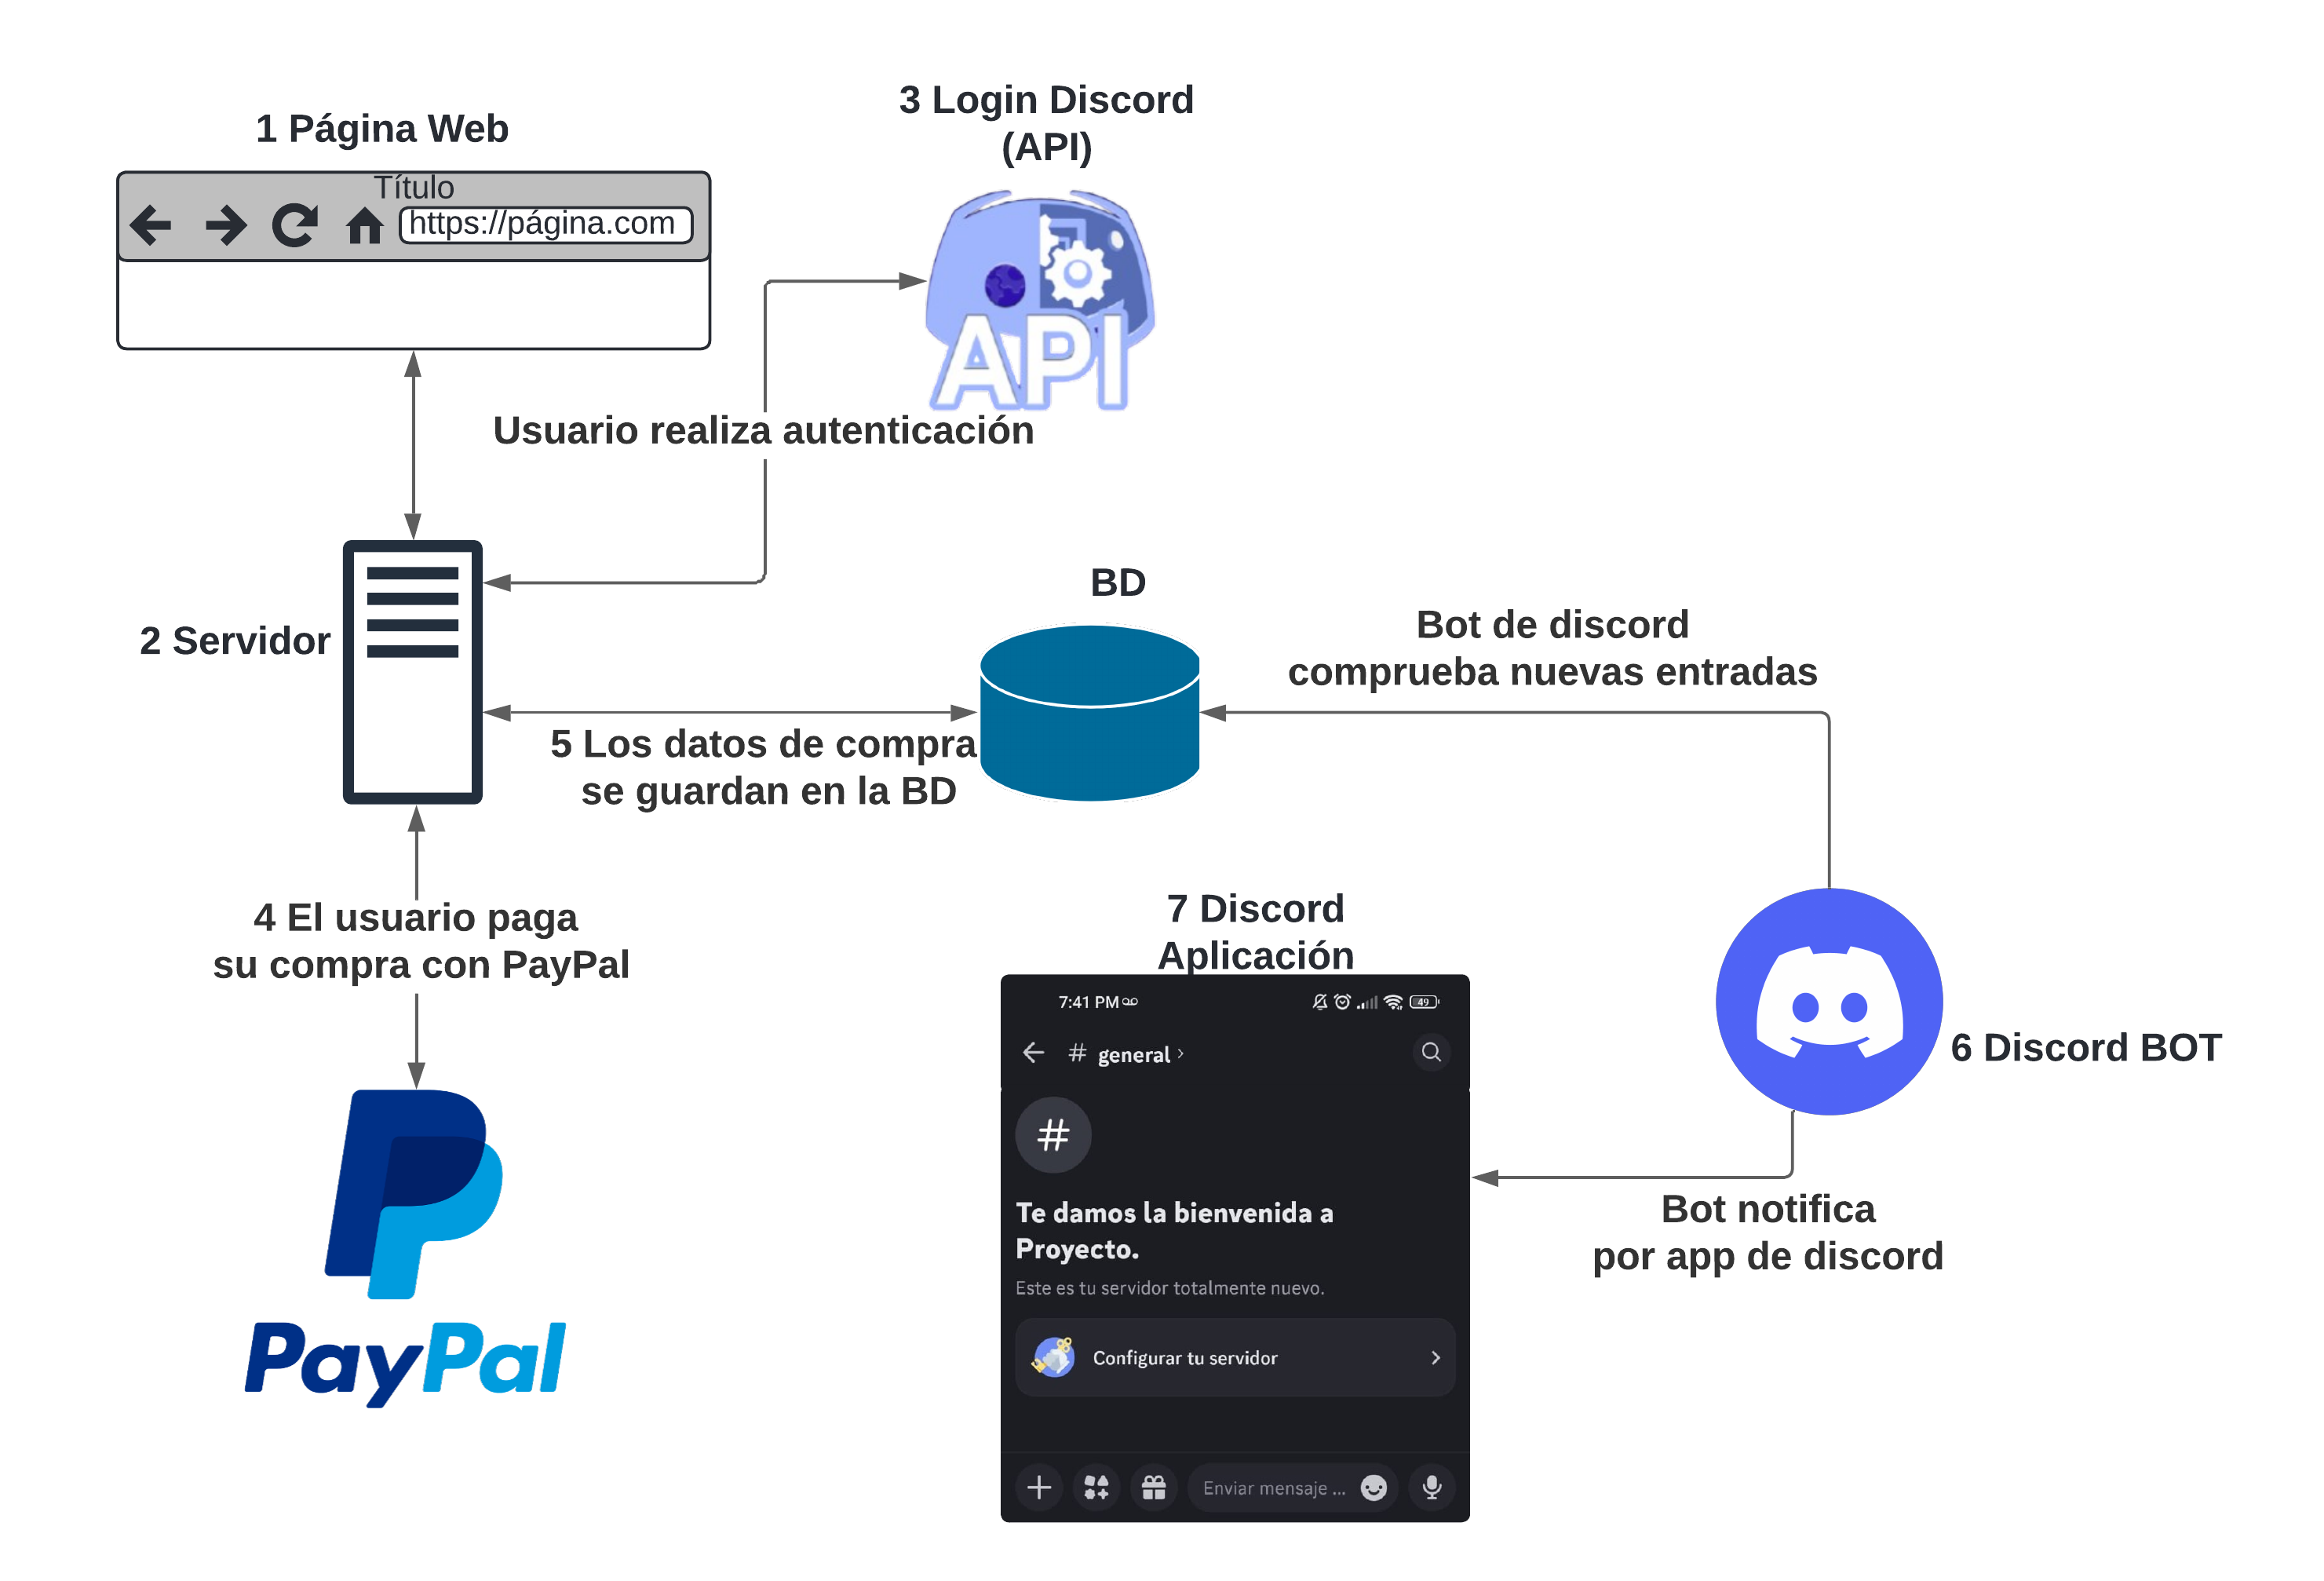
\includegraphics[width=0.8\textwidth]{./Diagramas/Diagramagen.png} % Ajustar el tamaño de la imagen y la ruta de la imagen
    \captionsetup{justification=centering}
    \caption{Diagrama general del sistema}  % Pie de imagen o descripción
    \label{fig:diagrama-general}  % Etiqueta para referenciar la imagen en el documento
\end{figure}


\vspace{1cm}
1.- El usuario podrá consultar los artículos a la venta en el sitio web.\\

2.- El servidor será el encargado de procesar todas las solicitudes que conectarán el front-end con toda la lógica. \\

3.- El sistema autenticará al usuario mediante su cuenta de Discord.\\

4.- Una vez teniendo artículos en el carrito de compra, el usuario podrá comprarlos y pagarlos mediante PayPal; deberá realizar una autenticación dentro de PayPal para poder acceder a su cuenta y realizar el pago.\\

5.- En la base de datos se guardarán todos los datos necesarios para autenticación, los datos de compra, y los artículos que se han colocado a la venta.\\

6.- El bot de Discord hará una función administrativa, esta será avisarle al administrador y al usuario comprador sobre su compra o próximas suscripciones. Estos avisos serán personales para cada usuario.\\

7.- Mediante Discord, el usuario recibirá las notificaciones que le enviará el bot; el usuario requiere un perfil dentro de Discord.\\

\newpage
\subsection{Diagrama Secuencial}
\begin{figure}[ht]  % Entorno figure para insertar la imagen
    \centering  % Centrar la imagen
    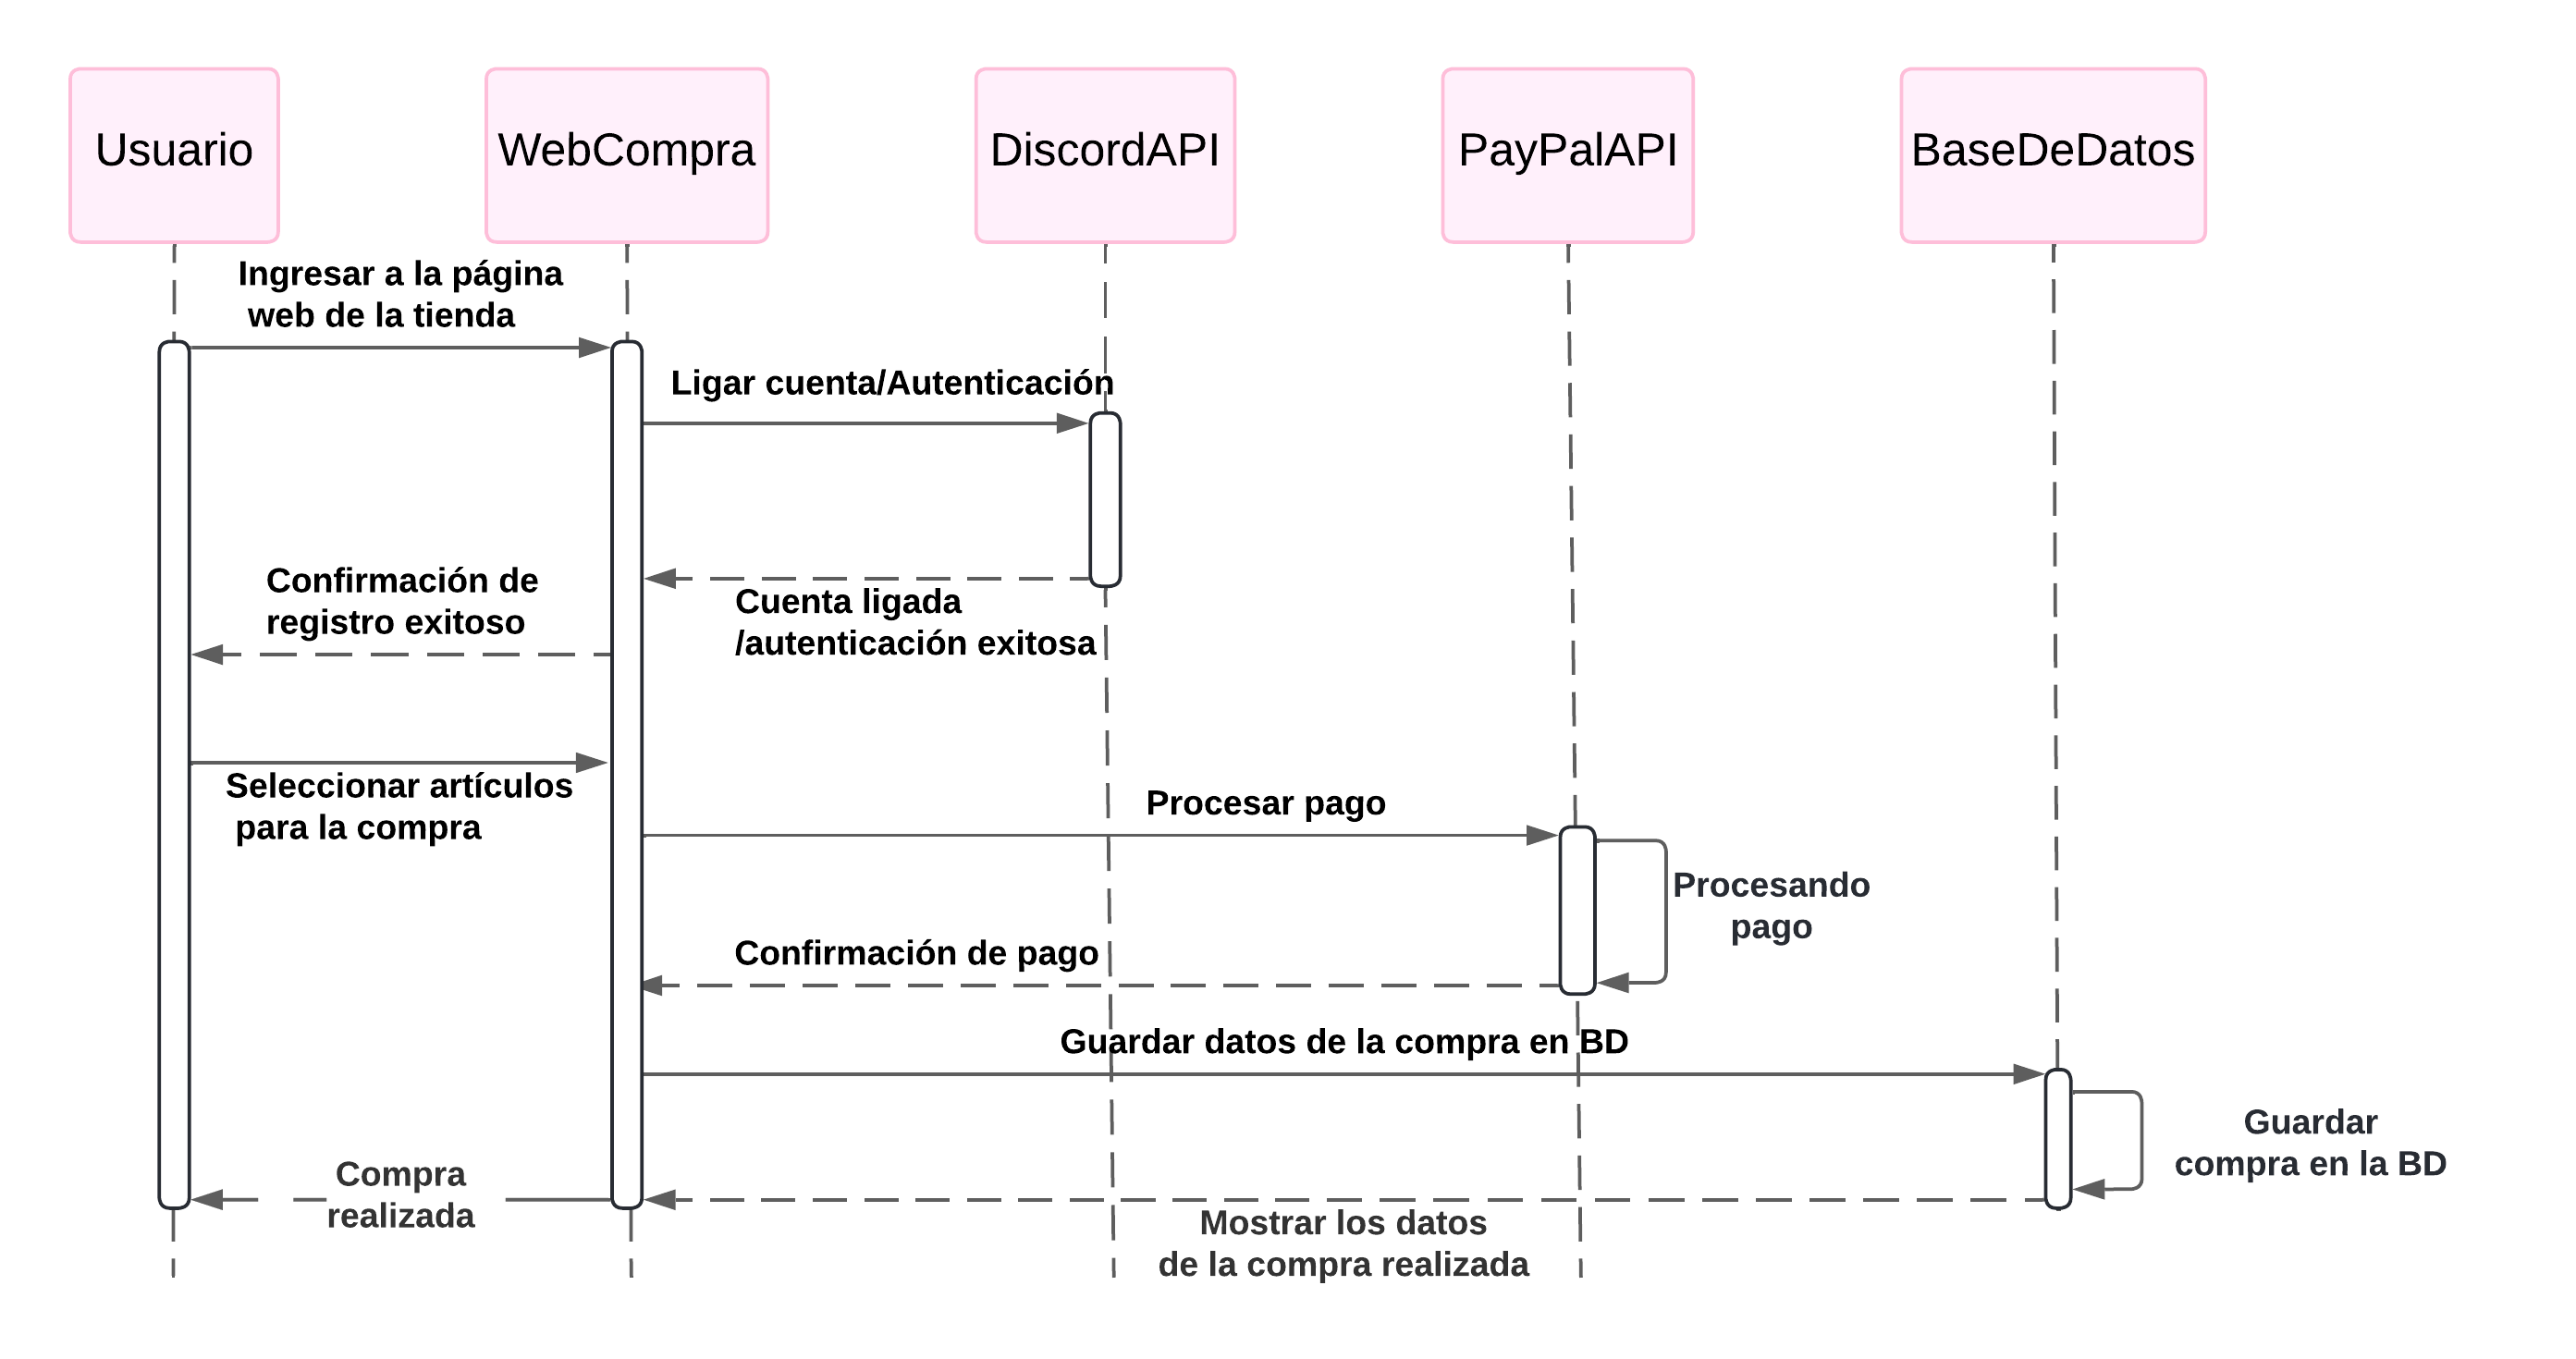
\includegraphics[width=1\textwidth]{./Diagramas/Diagramasec1.png} % Ajustar el tamaño de la imagen y la ruta de la imagen
    \captionsetup{justification=centering}
    \caption{Diagrama secuencial del sistema}  % Pie de imagen o descripción
    \label{fig:diagrama-secuencial1}  % Etiqueta para referenciar la imagen en el documento
\end{figure}
1.- El usuario deberá iniciar sesión, autenticarse en la página web para poder realizar compras.\\

2.- Una vez seleccionado el artículo de compra, se mandará al usuario a realizar su compra; se usará PayPal para realizar la validación de compra.\\

3.- La compra realizada se registrará en la base de datos.\\

4.- Se le mostrará al usuario un mensaje de compra exitosa.
\newpage

\begin{figure}[ht]  % Entorno figure para insertar la imagen
    \centering  % Centrar la imagen
    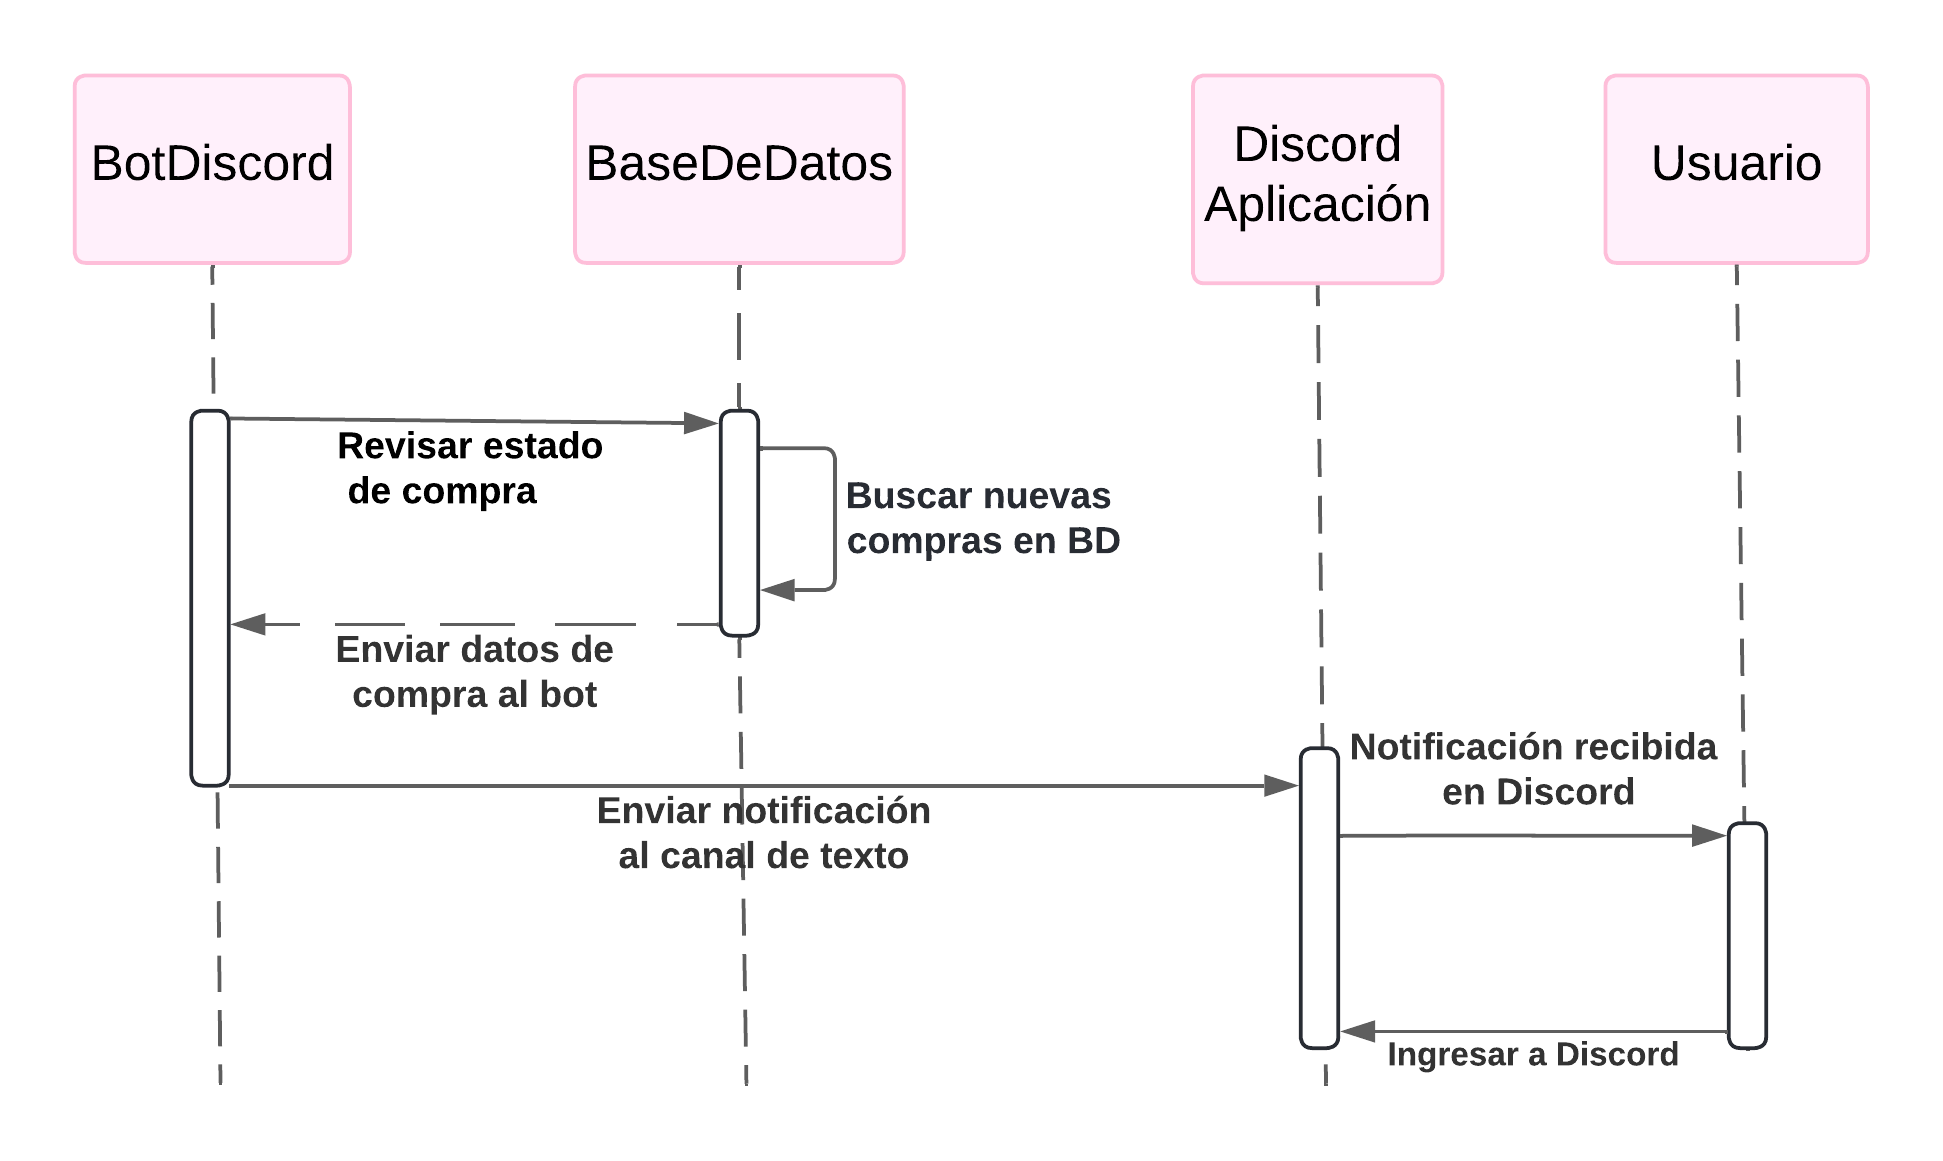
\includegraphics[width=1\textwidth]{./Diagramas/Diagramasec2.png} % Ajustar el tamaño de la imagen y la ruta de la imagen
    \captionsetup{justification=centering}
    \caption{Diagrama secuencial del sistema 2}  % Pie de imagen o descripción
    \label{fig:diagrama-secuencial2}  % Etiqueta para referenciar la imagen en el documento
\end{figure}

1.- El bot de Discord comprobará si hay nuevas entradas en la BD.\\

2.- El bot enviará los datos de compra vía Discord.\\

3.- El usuario comprador podrá ver los datos de su compra en el mensaje dejado por el bot.\\
\newpage

\subsection{Diagrama de la Base de Datos}
\begin{figure}[ht]  % Entorno figure para insertar la imagen
    \centering  % Centrar la imagen
    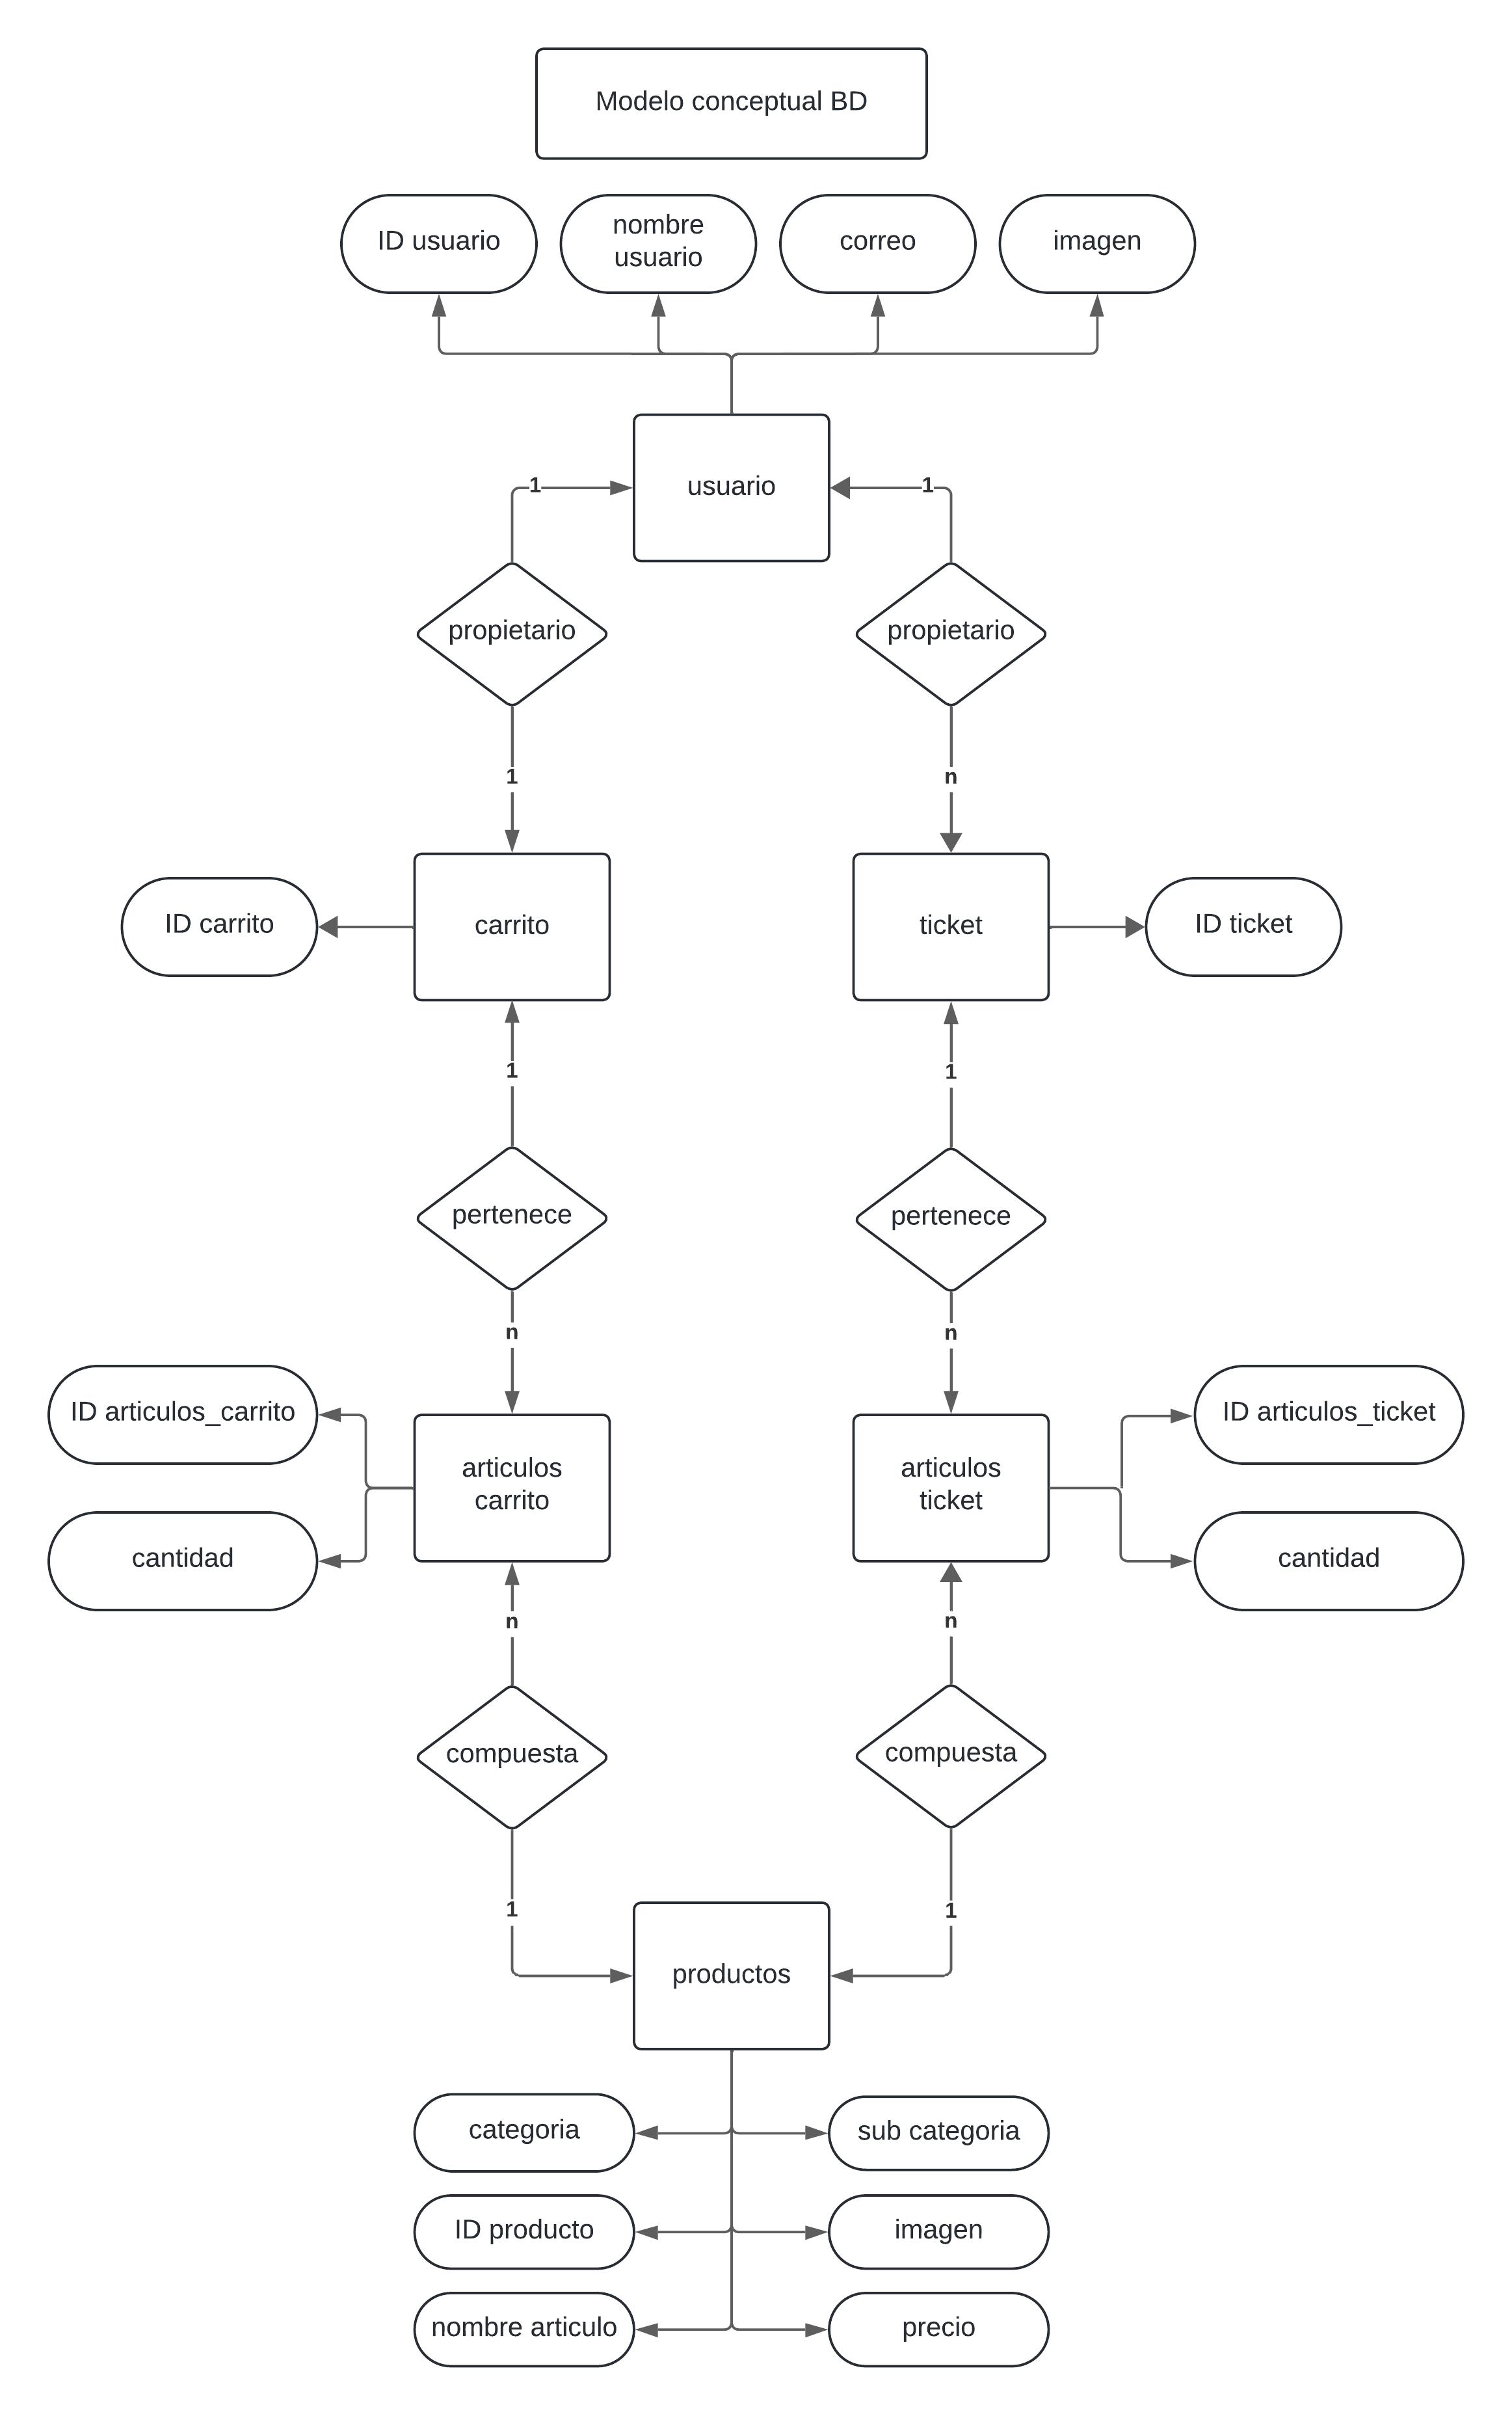
\includegraphics[width=0.5\textwidth]{./Diagramas/ModeloConsep.png} % Ajustar el tamaño de la imagen y la ruta de la imagen
    \captionsetup{justification=centering}
    \caption{Modelo Conceptual de la Base de Datos}  % Pie de imagen o descripción
    \label{fig:modelo-conceptual}  % Etiqueta para referenciar la imagen en el documento
\end{figure}

El diagrama de la figura 13 comienza con la entidad usuario, que contiene información básica como ID, nombre, correo e imagen. Cada usuario puede ser propietario de un carrito y puede tener muchos tickets, lo que implica que un mismo usuario puede realizar varias compras, pero solo tener un carrito activo a la vez.\\

El carrito está relacionado con el usuario mediante una relación de propiedad uno a uno, y contiene múltiples artículos del carrito, es decir, productos que el usuario ha agregado antes de comprar. Estos artículos tienen una cantidad y se relacionan con la entidad productos, lo cual indica qué producto específico se añadió y en qué cantidad.\\

Una vez que el usuario realiza una compra, se genera un ticket, también asociado al usuario, pero en una relación de uno a muchos (un usuario puede tener muchos tickets). El ticket contiene artículos del ticket, similares a los del carrito, con su respectiva cantidad y referencia al producto adquirido.\\

La entidad productos es el catálogo general, donde se guarda información de cada artículo como su ID, nombre, categoría, subcategoría, imagen y precio. Esta entidad es común tanto para los artículos del carrito como para los del ticket, ya que los productos son los mismos, solo cambian de estado según estén en proceso de compra (carrito) o ya comprados (ticket).\\ 

\begin{figure}[ht]  % Entorno figure para insertar la imagen
    \centering  % Centrar la imagen
    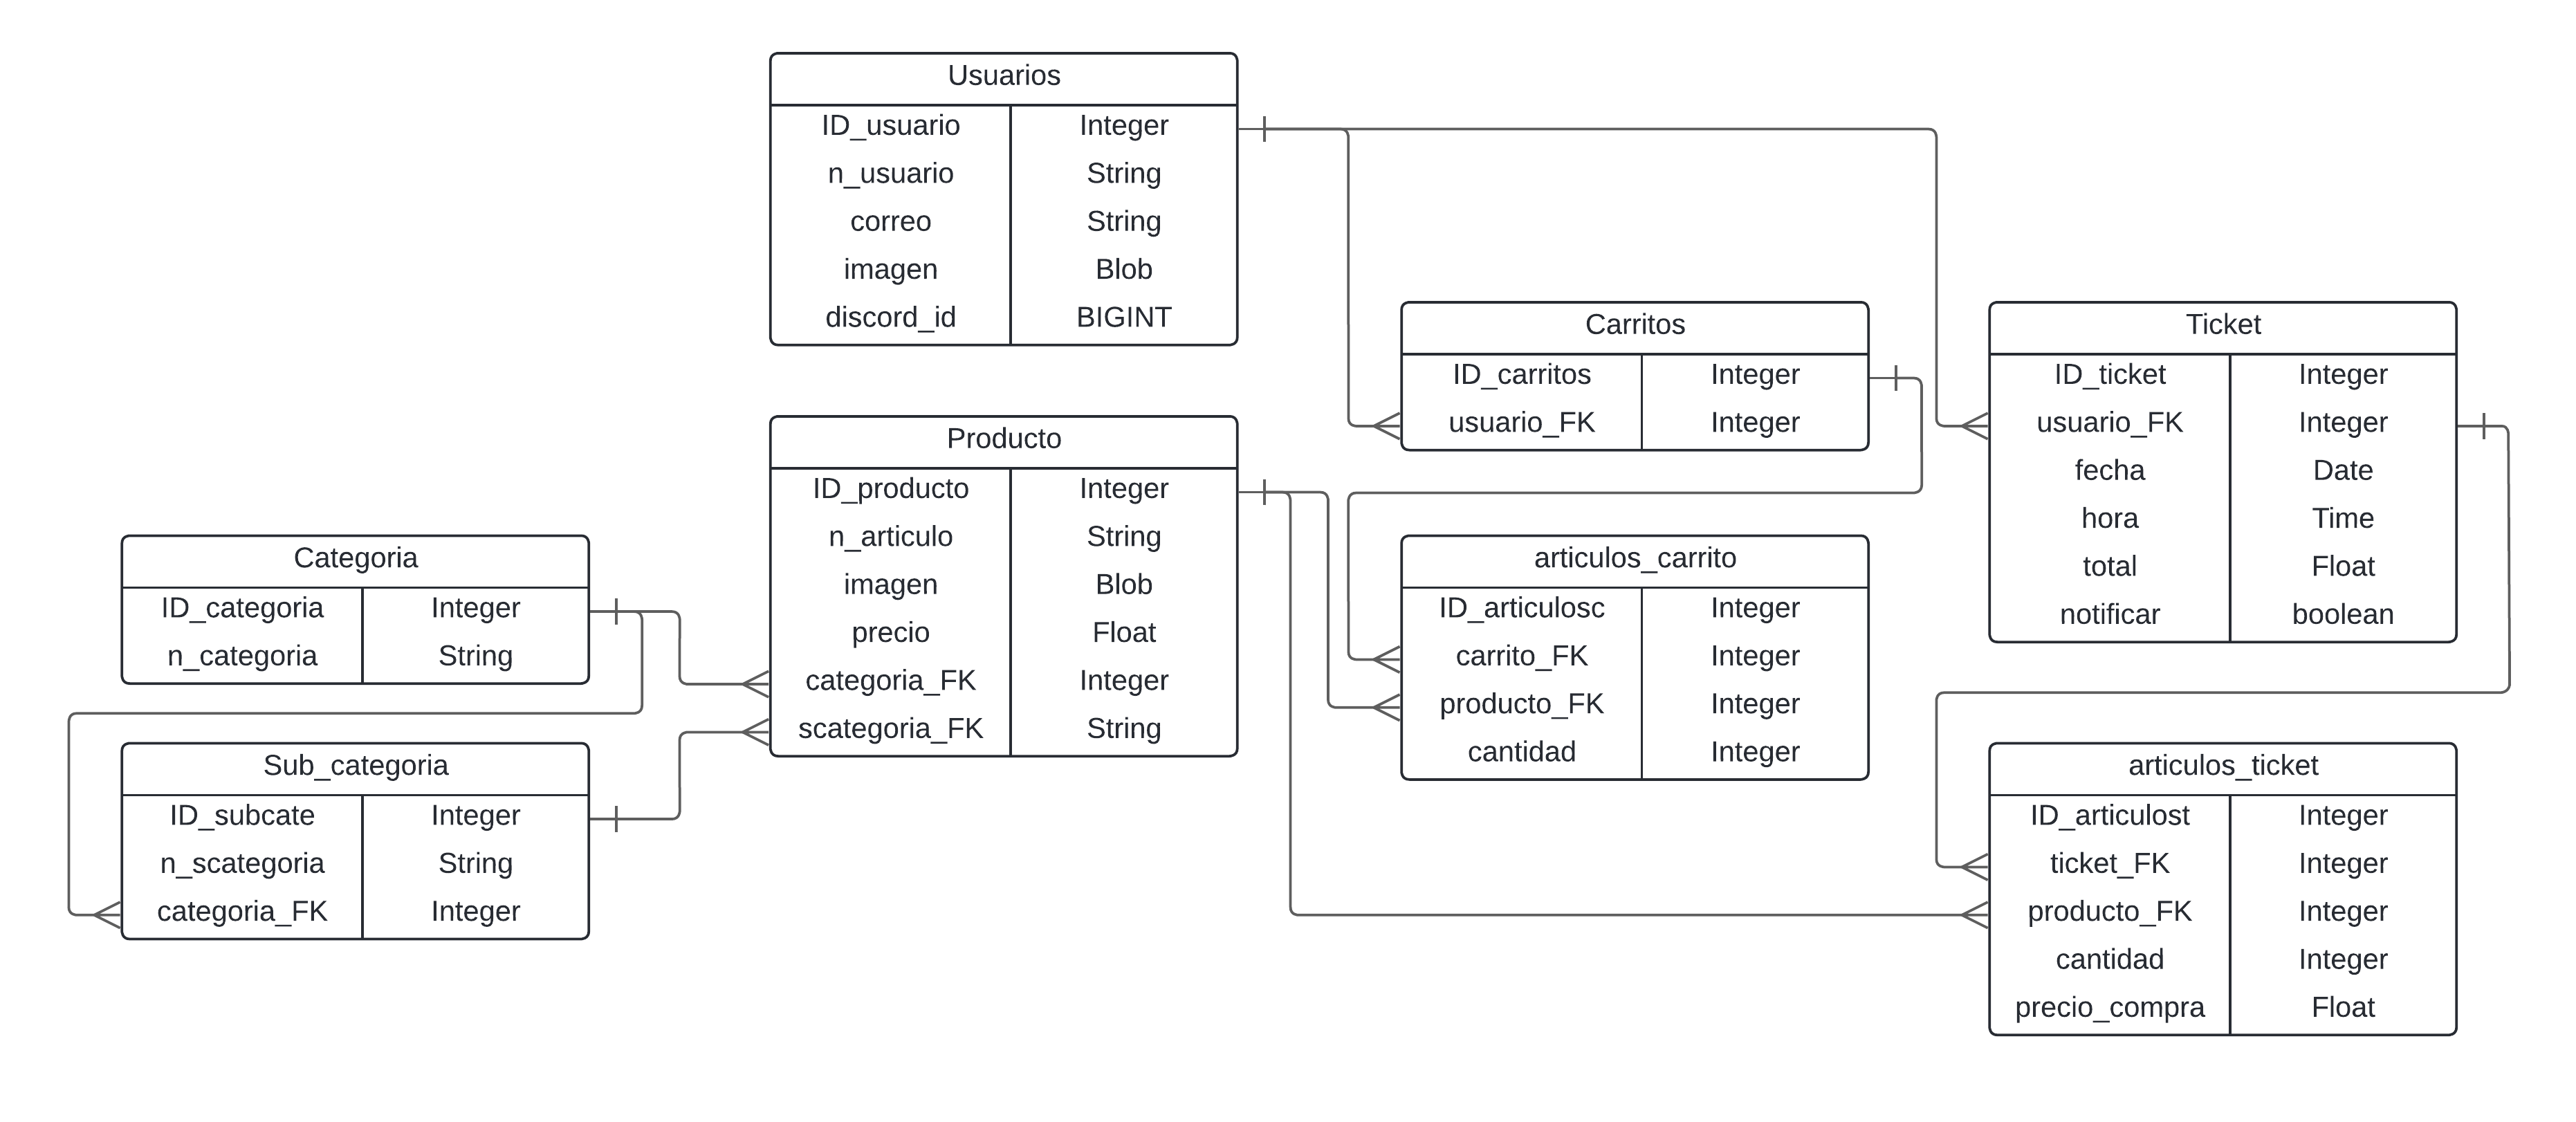
\includegraphics[width=1\textwidth]{./Diagramas/DiagramaBD.png} % Ajustar el tamaño de la imagen y la ruta de la imagen
    \captionsetup{justification=centering}
    \caption{Diagrama de la Base de Datos}  % Pie de imagen o descripción
    \label{fig:diagrama-bd}  % Etiqueta para referenciar la imagen en el documento
\end{figure}

En el diagrama de la figura 14 en base de datos, la entidad Usuarios almacena la información del cliente como ID, nombre, correo e imagen. Cada usuario puede tener un carrito (relación uno a uno) y también puede generar tickets de compra (relación uno a muchos).\\

El carrito está relacionado con el usuario mediante la clave foránea \textnormal{usuario\_FK} y contiene productos a través de la tabla \textnormal{articulos\_carrito}, donde se guarda qué producto fue agregado \textnormal{producto\_FK} y en qué cantidad.\\

Cuando se realiza una compra, se genera un ticket que también pertenece a un usuario (\textnormal{usuario\_FK}) y contiene información como fecha, hora, total de la compra y si se notificó. Los productos comprados se guardan en la tabla \textnormal{articulos\_ticket}, con su cantidad y el precio al momento de la compra (\textnormal{precio\_compra}), todo enlazado al ticket (\textnormal{ticket\_FK}) y al producto (\textnormal{producto\_FK}).\\

La entidad Producto almacena todos los artículos disponibles: su ID, nombre, imagen, precio y dos claves foráneas que lo conectan con su categoría y subcategoría (\textnormal{categoria\_FK} y \textnormal{scategoria\_FK}). Las categorías están organizadas en dos niveles, mediante las tablas Categoria y \textnormal{Sub\_categoria}, esta última relacionada con la primera a través de \textnormal{categoria\_FK}.


\newpage

\section{Desarrollo del sistema}
\subsection{APIS}
En esta sección se describen las APIs que formarán parte del sistema, tanto internas como externas. Las APIs (Interfaces de Programación de Aplicaciones) permiten la comunicación entre los diferentes componentes del sistema, como la tienda en línea y el bot de Discord, facilitando el intercambio de datos de forma estructurada y segura. A través de estas interfaces, el sistema podrá recibir eventos, enviar notificaciones y ejecutar funcionalidades clave que permiten la integración fluida entre la plataforma de e-commerce y Discord.

\subsubsection{API de PayPal}
1.- Creación de una cuenta de PayPal para negocios:
Debemos registrar una cuenta empresarial en el sitio web de PayPal. Esto permitirá vincular la cuenta a la tienda y recibir pagos directamente en ella.\\

2.- Configuración en el portal de desarrolladores de PayPal:
Acceder al portal de desarrolladores de PayPal (https://developer.paypal.com) para obtener credenciales de API, como:
- Client ID.
- Secret Key.
Estas credenciales son necesarias para autenticar las solicitudes desde la tienda hacia los servidores de PayPal.\\

3.- Integración de la API en la tienda:
Implementar la API de PayPal en el back-end de la tienda. Esto implica:
Configurar la solicitud de pago: indicar el monto de la compra, la moneda y los detalles del destinatario (cuenta de PayPal del vendedor).
Gestionar la respuesta de PayPal: verificar el estado del pago (éxito o error) y actualizar la información en la base de datos de la tienda.\\

4.- Incorporación de un botón de pago:
En el front-end, se utiliza el botón de PayPal, el cual es generado dinámicamente por la API o configurado manualmente con el código proporcionado por PayPal. Este botón redirige a los usuarios a la plataforma de PayPal para completar la transacción.\\

5.- Redirección tras el pago
Una vez completado el pago, el usuario es redirigido de regreso al sitio web de la tienda, donde se muestra una confirmación del pedido o un mensaje de error si la transacción falló.\\

Configuración\\
1. Crea una app en [PayPal Developer](https://developer.paypal.com/).\\
2. Obtén tu `Client ID` y `Client Secret` de sandbox.\\
3. Configura las credenciales en el backend:\\

estos coandos se recommenda colocarse en un archivo .env \\

\textnormal{PAYPAL\_CLIENT\_ID=...}\\
\textnormal{PAYPAL\_CLIENT\_SECRET=...}\\

En el back-end\\
\begin{lstlisting}[language=JavaScript, caption={Captura una orden de PayPal y genera el ticket}] 
POST /api/paypal/capture-order
Body: { orderId: string, total: number }
\end{lstlisting}

En el front-end\\
\begin{lstlisting}[language=JavaScript, caption={Al completar el pago con PayPal, enviar el orderId y total al backend}] 
axios.post(`${process.env.REACT_APP_BACKEND_URL}/api/paypal/capture-order`, {
  orderId,
  total
}, { withCredentials: true })
.then(res => {
  // Mostrar mensaje de exito y ticket
});
\end{lstlisting}


\subsubsection{API de Discord}
La API de Discord ermite a los usuarios autenticarse en la tienda usando su cuenta de Discord mediante OAuth2. Al autenticarse:\\

- El usuario es redirigido a Discord para autorizar la aplicación.\\
- Tras autorizar, Discord redirige al backend con un código temporal.\\
- El backend intercambia ese código por un token y obtiene los datos del usuario desde Discord.\\
- Si el usuario no existe en la base de datos, se crea automáticamente.\\
- Se genera una cookie de sesión (`user`) con los datos básicos del usuario (id, username (nombre de usuario), avatar, email).\\
- El frontend puede leer esta cookie (vía endpoint `/auth/user`) para mostrar el perfil y mantener la sesión.\\

Configuración:\\
Se realizó un registro de la aplicación en el [Portal de Desarrolladores de Discord]\\(https://discord.com/developers/applications) y obtener:\\
1 \textnormal{DISCORD\_CLIENT\_ID}\\
2 \textnormal{DISCORD\_CLIENT\_SECRET}\\
3 \textnormal{DISCORD\_REDIRECT\_URI} (ejemplo: `http://localhost:5000/auth/discord/callback`)\\




\begin{lstlisting}[language=JavaScript, caption={Se agregan estos valores al archivo `.env` del backend:}] 
DISCORD_CLIENT_ID=...
DISCORD_CLIENT_SECRET=...
DISCORD_REDIRECT_URI=http://localhost:5000/auth/discord/callback
FRONTEND_URL=http://localhost:3000
\end{lstlisting}
\newpage
Flujo y rutas principales de la API.\\

1. Iniciar login con Discord
GET /auth/login\\
- Redirige al usuario a la página de autorización de Discord.\\
- Se guarda un `state` aleatorio en una cookie para prevenir ataques CSRF.\\

2. Callback de Discord OAuth2\\
GET /auth/discord/callback\\
- Discord redirige a esta ruta tras la autorización.\\
- El backend valida el `state` o estado y obtiene el token de acceso.\\
- Se consulta la API de Discord para obtener los datos del usuario.\\
- Se guarda/actualiza el usuario en la base de datos.\\
- Se crea una cookie `user` con los datos básicos del usuario.\\
- Redirige al front-end de la tienda virtual.\\

3. Obtener usuario autenticado\\
GET /auth/user\\
- Devuelve los datos del usuario autenticado leyendo la cookie `user`.\\
- Si no hay cookie, responde 401.\\

4. Logout\\
POST /auth/logout\\
- Elimina la cookie `user` y termina la sesión.\\

\begin{lstlisting}[language=JavaScript, caption={La cookie que se genera para guardar los datos del usuario `user` contiene un JSON con:}] 
{
  "id": "discord_id",
  "username": "nombre_usuario",
  "avatar": "url_avatar_discord",
  "email": "correo@ejemplo.com"
}
\end{lstlisting}
Esta cookie es usada por el front-end para mostrar el perfil y por el back-end para identificar al usuario en operaciones como agregar al carrito o comprar.\\
\subsection{Bot de Discord}
\subsection{Punto de Venta}
\subsection{Base de Datos}

\section{Resultados}
\subsection{Interfaces del Punto de Venta}
\subsubsection{Interfaz de Inicio de Sesión por Discord}
\subsubsection{Interfaz de Página de Productos}
\subsubsection{Interfaz del Carrito y el Procesamiento de Tickets}

\subsection{funcionalidades del Bot}
\subsubsection{Creación de Comandos para Usuarios}
\subsubsection{Comprobación de Tickets Pendientes}
\subsubsection{Envío de Notificaciones por Canales Privados}

\section{Conclusiones}

\section{Referencias}

[1] PayPal, “Bienvenido a PayPal,” [En línea]. Disponible en: https://www.paypal.com/mx/webapps/mpp/welcome-to-paypal. [Accedido: 21-jun-2025].\\

[2] MEE6, “MEE6 - El bot de Discord más completo,” [En línea]. Disponible en: https://mee6.xyz/es. [Accedido: 21-jun-2025].\\

[3] R. Teja Rubio, “Proyecto Tienda Virtual: Uniformes Escolares,” TFC, Univ. Oberta de Catalunya, Ingeniería Técnica en Informática de Gestión, Ene. 2016. [En línea]. Disponible en: https://openaccess.uoc.edu/handle/10609/49345\\

[4] Facebook, “Marketplace de Facebook,” [En línea]. Disponible en: https://www.facebook.com/marketplace/. [Accedido: 21-jun-2025].\\

[5] AliExpress,  [En línea]. Disponible en: https://es.aliexpress.com/?spm=a2g0o.productlist.logo.1.6cbetR33tR33Kg. [Accedido: 21-jun-2025].\\



\end{document}